\documentclass[12pt, UTF8]{article}
\usepackage[a4paper, scale = 0.8]{geometry}
\usepackage{ctex}

\usepackage{enumitem}
\usepackage{listings}
\usepackage{xcolor}
\usepackage{color}
\definecolor{GrayCodeBlock}{RGB}{241, 241, 241}
%\definecolor{BlackText}{RGB}{110, 107, 94}
\definecolor{BlackText}{RGB}{0, 0, 0}
\definecolor{RedTypename}{RGB}{182, 86, 17}
\definecolor{GreenString}{RGB}{96, 172, 57}
\definecolor{PurpleKeyword}{RGB}{184, 84, 212}
\definecolor{GrayComment}{RGB}{170, 170, 170}
\definecolor{GoldDocumentation}{RGB}{180, 165, 45}
\lstset {
  columns = fullflexible, keepspaces = true, showstringspaces=false, breaklines = true, frame = single, framesep = 0pt, framerule = 0pt, framexleftmargin = 4pt, framexrightmargin = 4pt, framextopmargin = 5pt, framexbottommargin = 3pt, xleftmargin = 4pt, xrightmargin = 4pt,
  backgroundcolor = \color{GrayCodeBlock},
  basicstyle = \ttfamily\color{BlackText},
  keywordstyle = \color{PurpleKeyword},
  ndkeywordstyle = \color{RedTypename},
  stringstyle = \color{GreenString},
  commentstyle = \color{GrayComment}
}

\usepackage{graphicx}
\usepackage{amsmath}

\usepackage[colorlinks, linkcolor = red, anchorcolor = blue, citecolor = green]{hyperref}

\renewcommand\thesection{\arabic{section}}

\title{数据挖掘第六次作业}
\author{李晨昊 2017011466}
\begin{document}
\maketitle
\tableofcontents

\section{K-means聚类}

给定下列 13 个数据点:

(1,3); (1,2); (2,1); (2,2); (2,3); (3,2); (5,3); (4,3); (4,5); (5,4); (5,5); (6,4); (6,5)

使用 K-means 算法对它们进行聚类。令 k=2,初始中心点为(0,4)和(6,5),写出聚类过程。

\begin{enumerate}[label = Iter \arabic*:]
  \item
  \begin{itemize}
    \item (1, 3):距离(0, 4)为1.414,距离(6, 5)为5.385,选(0, 4)
    \item (1, 2):距离(0, 4)为2.236,距离(6, 5)为5.831,选(0, 4)
    \item (2, 1):距离(0, 4)为3.606,距离(6, 5)为5.657,选(0, 4)
    \item (2, 2):距离(0, 4)为2.828,距离(6, 5)为5.000,选(0, 4)
    \item (2, 3):距离(0, 4)为2.236,距离(6, 5)为4.472,选(0, 4)
    \item (3, 2):距离(0, 4)为3.606,距离(6, 5)为4.243,选(0, 4)
    \item (5, 3):距离(0, 4)为5.099,距离(6, 5)为2.236,选(6, 5)
    \item (4, 3):距离(0, 4)为4.123,距离(6, 5)为2.828,选(6, 5)
    \item (4, 5):距离(0, 4)为4.123,距离(6, 5)为2.000,选(6, 5)
    \item (5, 4):距离(0, 4)为5.000,距离(6, 5)为1.414,选(6, 5)
    \item (5, 5):距离(0, 4)为5.099,距离(6, 5)为1.000,选(6, 5)
    \item (6, 4):距离(0, 4)为6.000,距离(6, 5)为1.000,选(6, 5)
    \item (6, 5):距离(0, 4)为6.083,距离(6, 5)为0.000,选(6, 5)
  \end{itemize}
  聚为两类,分别为\{(1, 3), (1, 2), (2, 1), (2, 2), (2, 3), (3, 2)\}和\{(5, 3), (4, 3), (4, 5), (5, 4), (5, 5), (6, 4), (6, 5)\},中心点分别为(1.833, 2.167)和(5, 4.143)。
  \item
  \begin{itemize}
    \item (1, 3):距离(1.833, 2.167)为1.179,距离(5, 4.143)为4.160,选(1.833, 2.167)
    \item (1, 2):距离(1.833, 2.167)为0.850,距离(5, 4.143)为4.538,选(1.833, 2.167)
    \item (2, 1):距离(1.833, 2.167)为1.179,距离(5, 4.143)为4.345,选(1.833, 2.167)
    \item (2, 2):距离(1.833, 2.167)为0.236,距离(5, 4.143)为3.687,选(1.833, 2.167)
    \item (2, 3):距离(1.833, 2.167)为0.850,距离(5, 4.143)为3.210,选(1.833, 2.167)
    \item (3, 2):距离(1.833, 2.167)为1.179,距离(5, 4.143)为2.931,选(1.833, 2.167)
    \item (5, 3):距离(1.833, 2.167)为3.274,距离(5, 4.143)为1.143,选(5, 4.143)
    \item (4, 3):距离(1.833, 2.167)为2.321,距离(5, 4.143)为1.519,选(5, 4.143)
    \item (4, 5):距离(1.833, 2.167)为3.567,距离(5, 4.143)为1.317,选(5, 4.143)
    \item (5, 4):距离(1.833, 2.167)为3.659,距离(5, 4.143)为0.143,选(5, 4.143)
    \item (5, 5):距离(1.833, 2.167)为4.249,距离(5, 4.143)为0.857,选(5, 4.143)
    \item (6, 4):距离(1.833, 2.167)为4.552,距离(5, 4.143)为1.010,选(5, 4.143)
    \item (6, 5):距离(1.833, 2.167)为5.039,距离(5, 4.143)为1.317,选(5, 4.143)
  \end{itemize}
  聚类结果与前一次迭代相同,迭代中止。
\end{enumerate}

综上,聚类结果为\{(1, 3), (1, 2), (2, 1), (2, 2), (2, 3), (3, 2)\}和\{(5, 3), (4, 3), (4, 5), (5, 4), (5, 5), (6, 4), (6, 5)\}。

\section{层次聚类}

使用表中的相似度矩阵进行 Min 聚类和 Max 聚类,分别绘制树状图显示结果。树状图应当清楚地显示合并的次序。

\newpage

\begin{table}[htbp]
  \begin{center}
  相似度矩阵\\
  \begin{tabular}{|c|c|c|c|c|c|}
    \hline
    & P1   & P2   & P3   & P4   & P5   \\ \hline
    P1 & 1.00 & 0.10 & 0.41 & 0.55 & 0.35 \\ \hline
    P2 & 0.10 & 1.00 & 0.64 & 0.47 & 0.98 \\ \hline
    P3 & 0.41 & 0.64 & 1.00 & 0.44 & 0.85 \\ \hline
    P4 & 0.55 & 0.47 & 0.44 & 1.00 & 0.76 \\ \hline
    P5 & 0.35 & 0.98 & 0.85 & 0.76 & 1.00 \\ \hline
  \end{tabular}
\end{center}
\end{table}

\begin{itemize}
  \item Min
  \begin{center}
    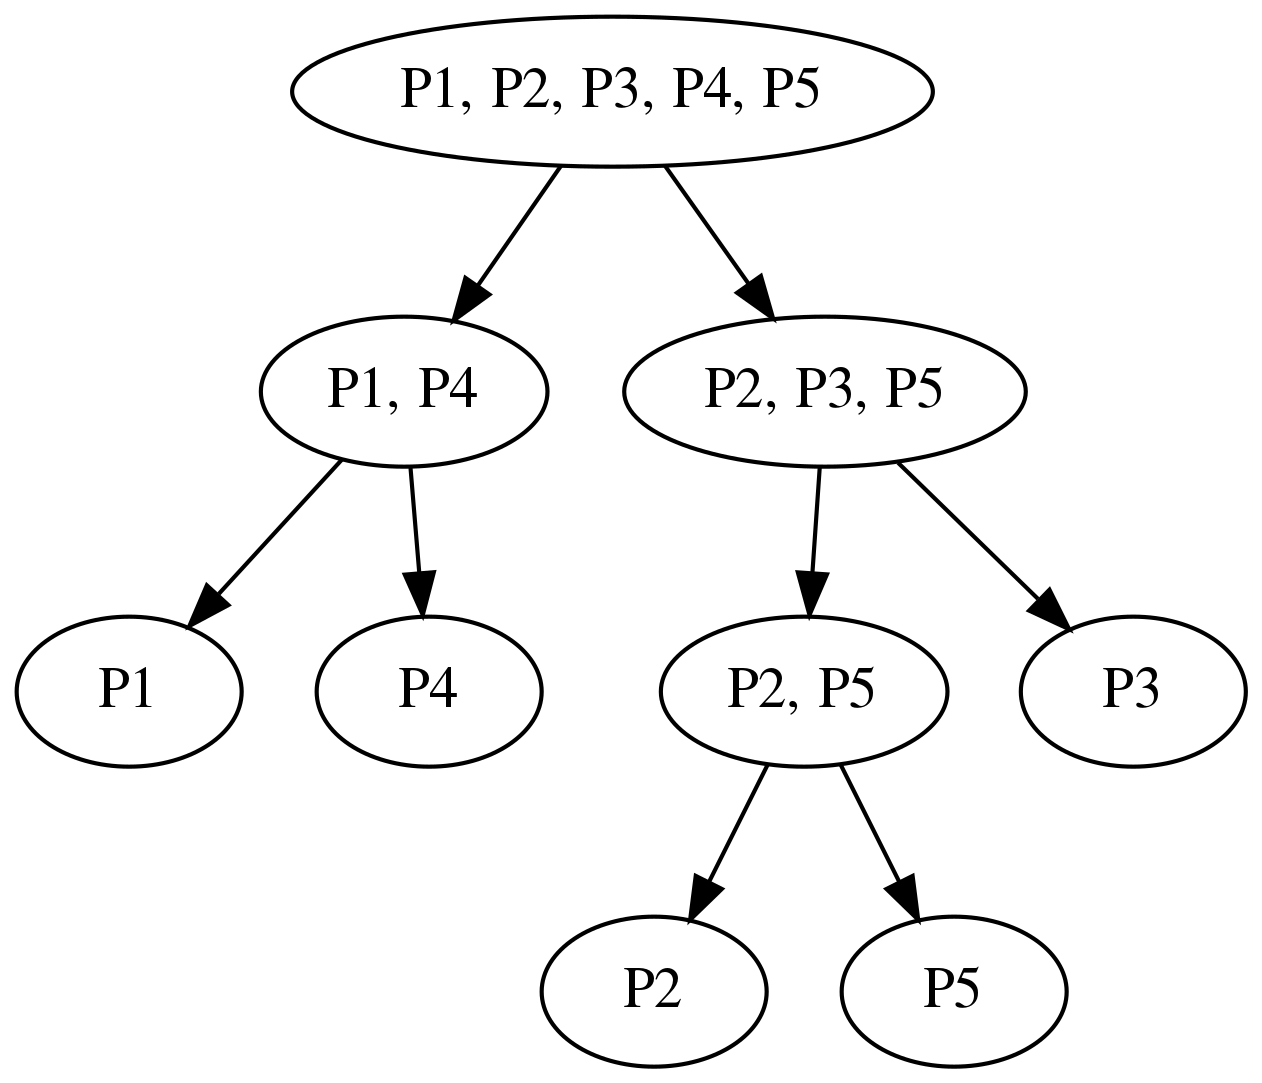
\includegraphics[width=0.4\textwidth]{min_hierarchical.png}
  \end{center}
  \item Max
  \begin{center}
    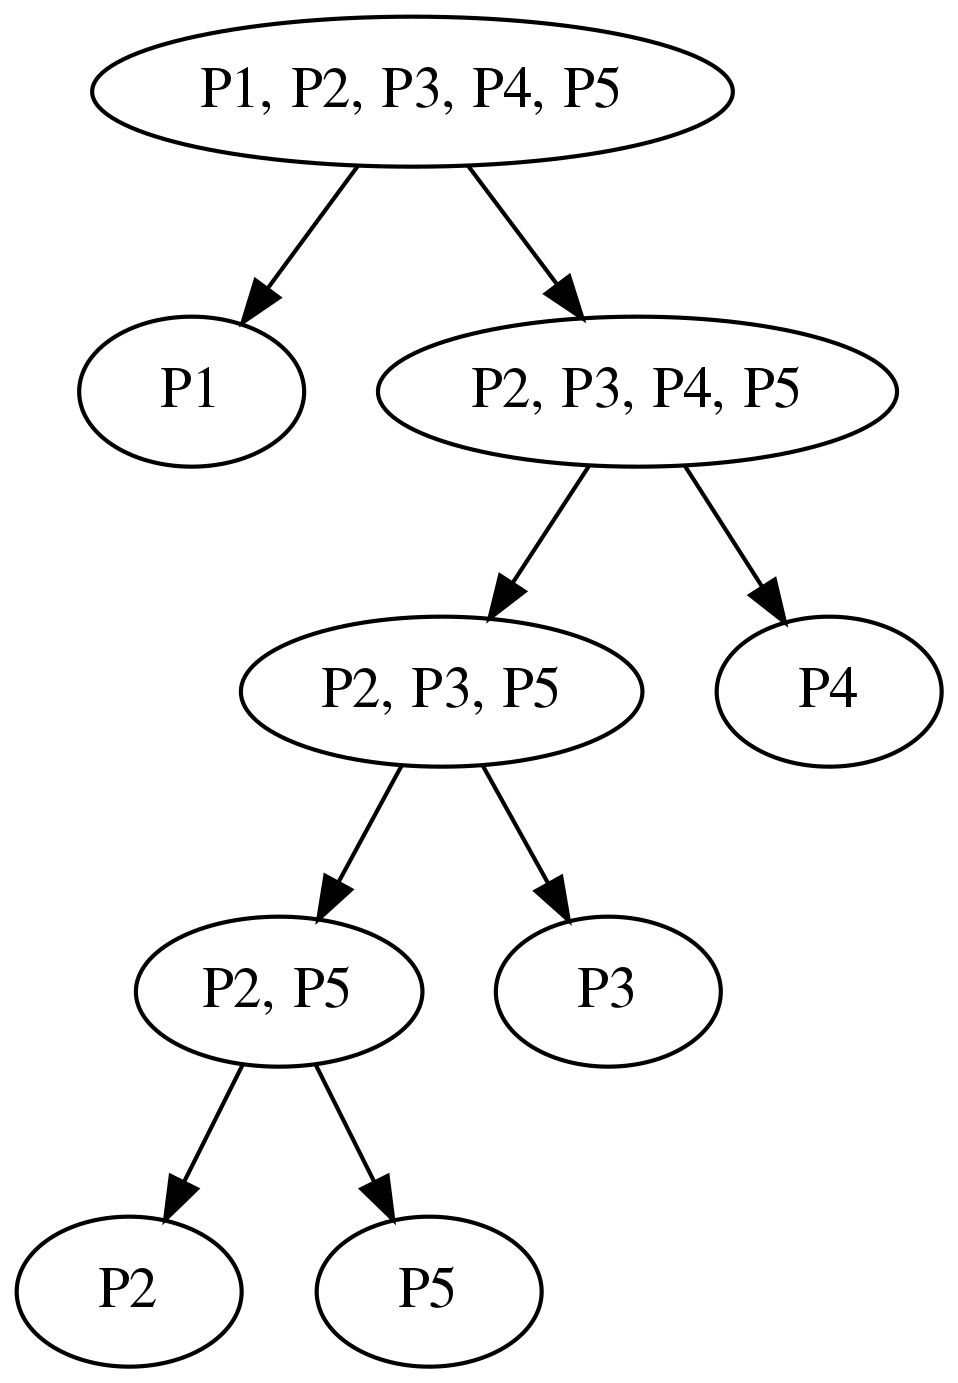
\includegraphics[width=0.3\textwidth]{max_hierarchical.png}
  \end{center}
\end{itemize}

\section{比较K-means和DBSCAN}

为了简化比较,假定对于K-Means和DBSCAN都没有距离的限制,并且DBSCAN总是将于若干个核心点相关联的边界点指派到最近的核心点。至少写出四点。(提示:可以从复杂度、离群点、参数等方面考虑。)

\begin{enumerate}
  \item K-means的时间复杂度为$O(tkn)$,其中$n$是对象个数,$k$是簇的个数,$t$是迭代次数,一般来说有$t, k \ll n$;DBSCAN最坏情况下时间复杂度为$O(n^2)$,其中$n$是对象个数。这样来看一般K-means更高效一些.
  \item K-means受数据噪音和离群点影响较大,DBSCAN则更加鲁棒。
  \item K-means需要用户指定簇的个数作为参数,DBSCAN则不需要,而是运行中自动确定簇的个数。
  \item K-means很难处理非凸形状的簇,DBSCAN可以发现任意形状的簇。
\end{enumerate}

\section{比较EM聚类和K-Means}

下图显示具有两个簇的二维点集的聚类。左边的簇(点用星号标记)多少有点散开,而右边的簇(点用圆标记)是紧凑的。在紧凑簇的右边有一个单独的点(用箭头指出)属于散开的簇。该簇的中心比紧凑簇的中心远得多。解释为什么用 EM聚类是可能的,但是用 K-Means 聚类不可能。

\begin{center}
  具有两个不同密度的簇的二维点集的 EM 聚类 \\
  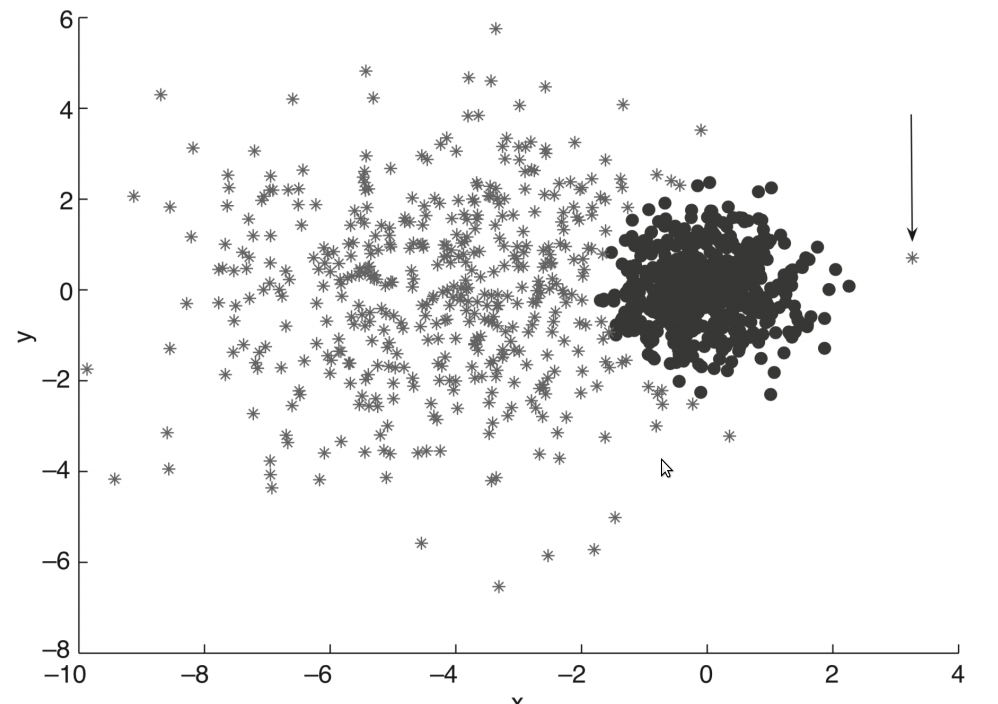
\includegraphics[width=0.5\textwidth]{t4.png}
\end{center}

这个聚类结果可能是EM聚类生成的,因为EM聚类基于高斯分布$f(x) = \frac{1}{\sqrt{2\pi}\sigma}e^{-\frac{(x-\mu)^2}{2\sigma^2}}$,因为左边的簇更分散,所以左边的簇对应的高斯分布的$\sigma$大于右边的簇的$\sigma$。因此即使右边的单独的点距离右边的簇更近(即$(x-\mu_{\text{左}})^2 > (x-\mu_{\text{右}})^2$),仍有可能有$\frac{(x-\mu_{\text{左}})^2}{2\mu_{\text{左}}^2} < \frac{(x-\mu_{\text{右}})^2}{2\mu_{\text{右}}^2}$,即它属于左边的簇的概率仍然可能更高一些。

这个聚类结果不可能是K-Means 聚类生成的,因为右边的单独的点距离右边的簇的中心比距离自身所在簇的中心更近,只要再进行一次迭代,最后一次迭代的时候不可能将它划分到左边的簇,因此这不可能是K-Means 聚类的最终结果。

\section{如何选择合适的聚类算法}

在确定使用哪种类型的聚类算法时,需要考虑各种各样的因素。简单分析选择合适的聚类算法时,涉及对哪些问题的考虑。至少写出四点。

\begin{enumerate}
  \item 时间和空间效率。例如K-Means算法简单且效率较高,如果用它就能达到不错的效果(即数据集中没有K-Means难以处理的哪几个特征),那么可以优先使用它,而无需采用更复杂的算法。或者如果数据规模很大,那么有些复杂度较高的算法即使效果好,也无法在实际工程中使用。
  \item 鲁棒性,包括算法对数据中的噪音和参数设置的敏感性。例如K-Means受噪音影响较大,而且很容易受到初始聚类的影响,一些种类的层次聚类也受噪音影响较大,而DBSCAN的鲁棒性则更好。如果实际数据中有较多的噪音,就应该选用鲁棒性更好的算法。
  \item 数据的特征。不同的算法对数据特征有不同的要求,例如K-Means要求数据必须有均值的概念,所以很难处理标签数据,层次聚类只要求数据有相似度的概念。如果实际数据不具备某一算法必要的特征,那么就很难应用它。
  \item 数据集的特征,也就是簇的形状和大小等特征。例如K-Means和一些种类的层次聚类很难处理非凸形状的簇,而DBSCAN可以处理不同大小和形状的簇。这一点一般来说很难事先知道,很多时候我们都是看着聚类的结果去讨论数据集的特征的,所以只能多尝试几种聚类算法,根据结果来调整。
\end{enumerate}

\end{document}